\documentclass[oneside,14pt]{extarticle}
\usepackage{cmap}
\usepackage[utf8]{inputenc}
\usepackage[english,ukrainian]{babel}
\usepackage{graphicx}
\usepackage{geometry}
\usepackage{listings}
\usepackage{float}
\usepackage{amsmath}
\usepackage{subfig}
\usepackage{tempora}
\geometry{
	a4paper,
	left=20mm,
	right=20mm,
	top=15mm,
	bottom=15mm,
}
\lstset{
	language=c,
	tabsize=4,
	keepspaces,
	showstringspaces=false,
	frame=single,
	breaklines,
	language=C,
}
\graphicspath{ {./pictures} }
\setlength{\parindent}{4em}

\newcommand\subject{Системне адміністрування}
\newcommand\lecturer{професор кафедри ПЗ\\Фечан А.В.}
\newcommand\teacher{професор кафедри ПЗ\\Фечан А.В.}
\newcommand\mygroup{ПЗ-42}
\newcommand\lab{5}
\newcommand\theme{Аудит. Політики аудиту. Робота з журналом безпеки
	Windows}
\newcommand\purpose{Ознайомлення з політиками та налаштуванням аудиту,
	аналізом безпеки системи шляхом вивчення журналу подій в Windows 10.
	Навчитись проводити аудит локальної системи та працювати з журналом
	безпеки Windows}

\begin{document}
\begin{normalsize}
	\begin{titlepage}
		\thispagestyle{empty}
		\begin{center}
			\textbf{МІНІСТЕРСТВО ОСВІТИ І НАУКИ УКРАЇНИ\\
				НАЦІОНАЛЬНИЙ УНІВЕРСИТЕТ "ЛЬВІВСЬКА ПОЛІТЕХНІКА"}
		\end{center}
		\begin{flushright}
			\textbf{ІКНІ}\\
			Кафедра \textbf{ПЗ}
		\end{flushright}
		\vspace{80pt}
		\begin{center}
			\textbf{ЗВІТ}\\
			\vspace{10pt}
			до лабораторної роботи № \lab\\
			\textbf{на тему}: <<\textit{\theme}>>\\
			\textbf{з дисципліни}: <<\subject>>
		\end{center}
		\vspace{80pt}
		\begin{flushright}
			
			\textbf{Лектор}:\\
			\lecturer\\
			\vspace{28pt}
			\textbf{Виконав}:\\
			
			студент групи \mygroup\\
			Коваленко Д.М.\\
			\vspace{28pt}
			\textbf{Прийняв}:\\
			
			\teacher\\
			
			\vspace{28pt}
			«\rule{1cm}{0.15mm}» \rule{1.5cm}{0.15mm} 2024 р.\\
			$\sum$ = \rule{1cm}{0.15mm}……………\\
			
		\end{flushright}
		\vspace{\fill}
		\begin{center}
			\textbf{Львів — 2024}
		\end{center}
	\end{titlepage}
		
	\begin{description}
		\item[Тема.] \theme.
		\item[Мета.] \purpose.
	\end{description}

    \section*{Лабораторне завдання}
	\begin{enumerate}
		\item Відкрити оснастку mmc "Групова політика". Перейти в гілку
		"Політика аудита", включити аудит доступу до об’єктів. Після цього у
		властивостях безпеки об’єкту, за яким повинно проводитись спостереження
		(папки чи файлу), перейти у вкладку "Аудит". та увімкнути аудит для визначених
		суб’єктів безпеки та їх активності (наприклад видалення). (Переконатись, що без
		налаштування аудиту на об’єкті файлової системи записів в журнал не
		відбувається – п. 2.) Виконати умови аудиту (тобто дії над цим об’єктом та тим
		користувачем для яких налаштовано аудит).
		\item Створимо в щойно налаштованій папці довільний текстовий файл
		(наприклад, audit.txt). Увійдемо до системи від користувача newuser і видалимо
		його. Повернемося до облікового запису адміністратора і переконаємося, що
		з’явився відповідний запис в журналі подій.
		\item В політиках аудиту увімкнути аудит зміни політики та системних
		подій. Виконати умови аудиту (наприклад змінити системний час). В журналі
		безпеки відстежити записи про ці події. Увімкнути аудит управління обліковими
		записами користувачів; відключити обліковий запис існуючого користувача,
		створити нового користувача, задати пароль користувачу. В журналі безпеки
		відстежити записи про ці події. Увімкнути аудит входу в систему; вийти зі
		системи та зайти під іншим користувачем. В журналі безпеки знайти записи
		категорії "Вхід/Вихід" та відстежити записи про ці події.
		\item У контекстному меню журналу безпеки вибрати пункт
		"Властивості". Задати якнайменший розмір журналу та політику "Не затирати
		події". Після цього в редакторі об’єкту групової політики (гілка "Параметри
		безпеки" (рис. 22)) включити параметр політики " Аудит: негайне відключення
		системи, якщо неможливо внести в журнал запису про аудит безпеки".
		Заповнити журнал аудиту увімкнувши політики та виконавши достатню
		кількість дій, що підлягають аудиту. Якщо це виконувалось користувачем з
		адміністративними повноваженнями, спробувати увійти в систему як звичайний
		користувач. Переконатись у неможливості входу в систему через переповненість
		журналу аудиту. Увійти як адміністратор; вимкнути увесь аудит. В контекстному
		меню журналу безпеки вибрати пункт "Затерти всі події" для очищення журналу.
		Чи усі події вдалося видалити? Чи з’явились нові записи?
	\end{enumerate}

	\section*{Хід роботи}
	
	\begin{figure}[H]
		\centering
		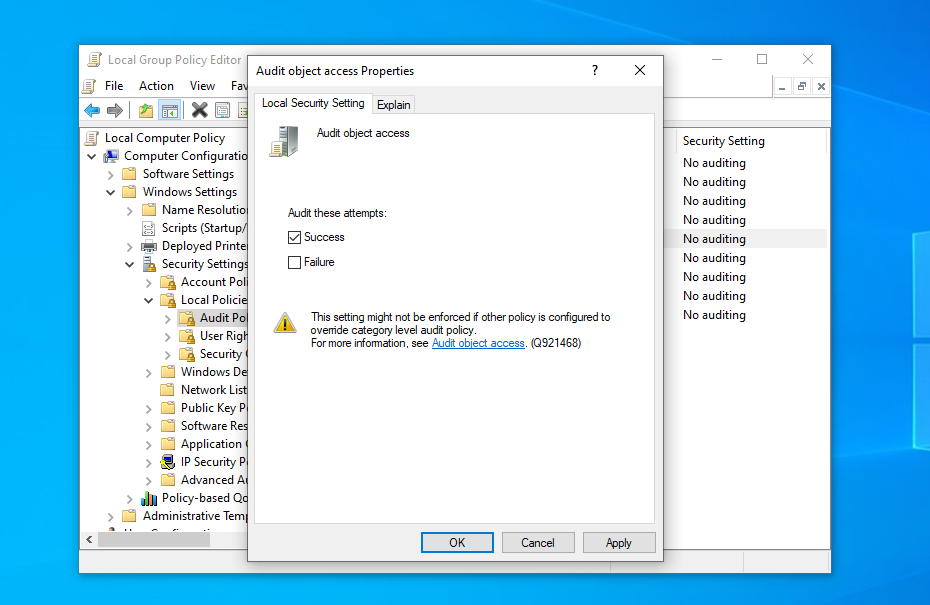
\includegraphics[width=\columnwidth]{1}
		\caption{Встановлення групової політики аудиту}
	\end{figure}
	
	\begin{figure}[H]
		\centering
		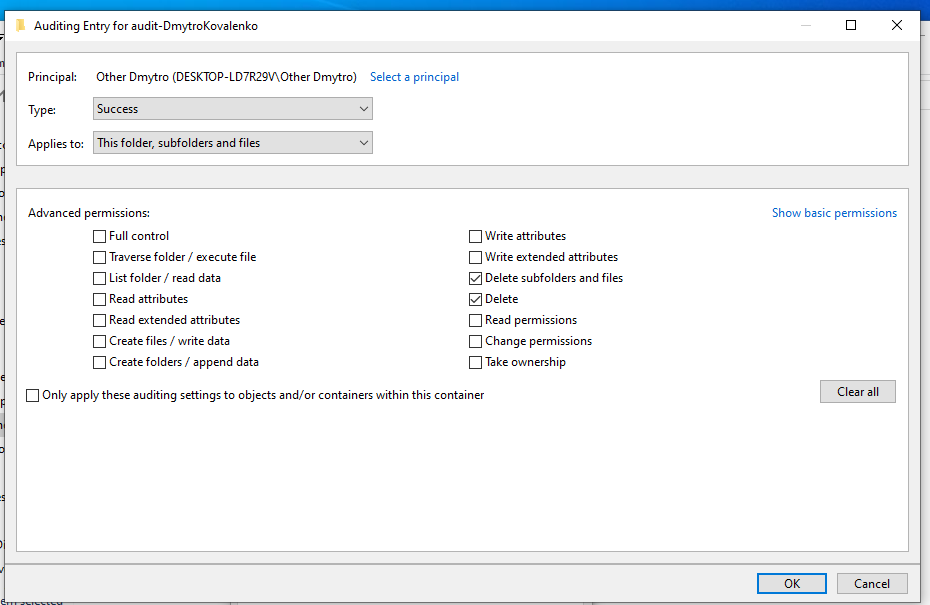
\includegraphics[width=\columnwidth]{2}
		\caption{Встановлення групової політики аудиту}
	\end{figure}
	\begin{figure}[H]
		\centering
		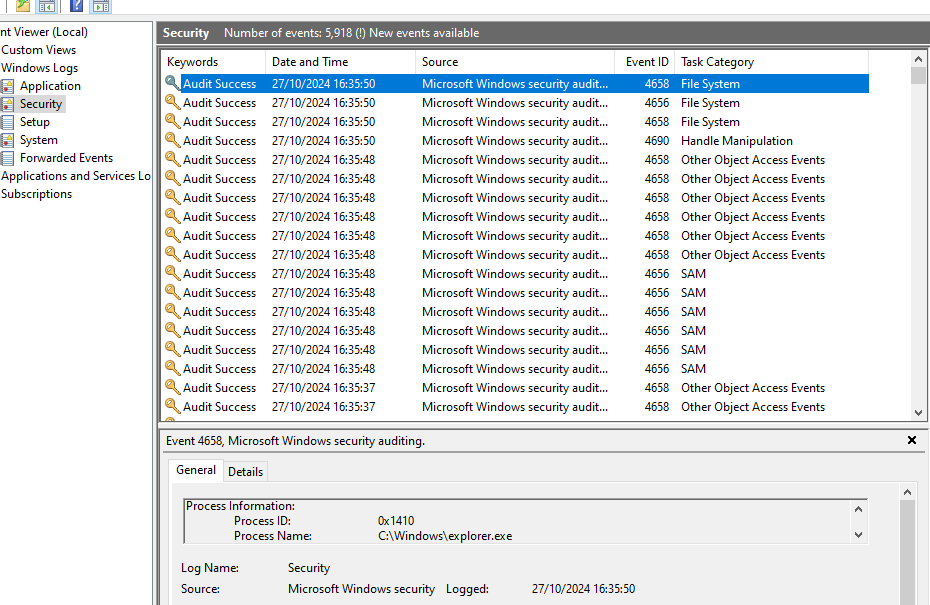
\includegraphics[width=\columnwidth]{3}
		\caption{Запис в журналі аудиту}
	\end{figure}
		\begin{figure}[H]
		\centering
		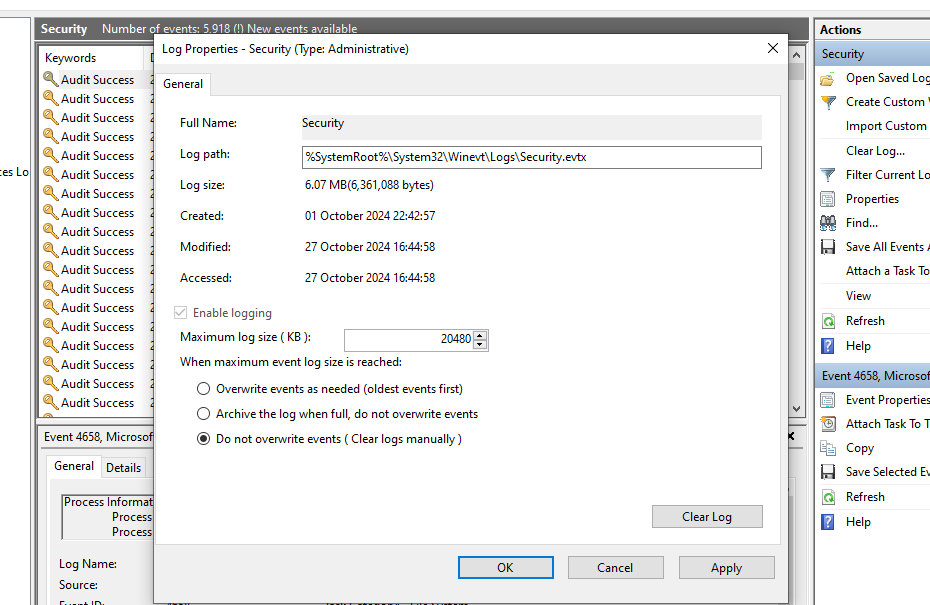
\includegraphics[width=\columnwidth]{4}
		\caption{Встановлення опції}
	\end{figure}
		\begin{figure}[H]
		\centering
		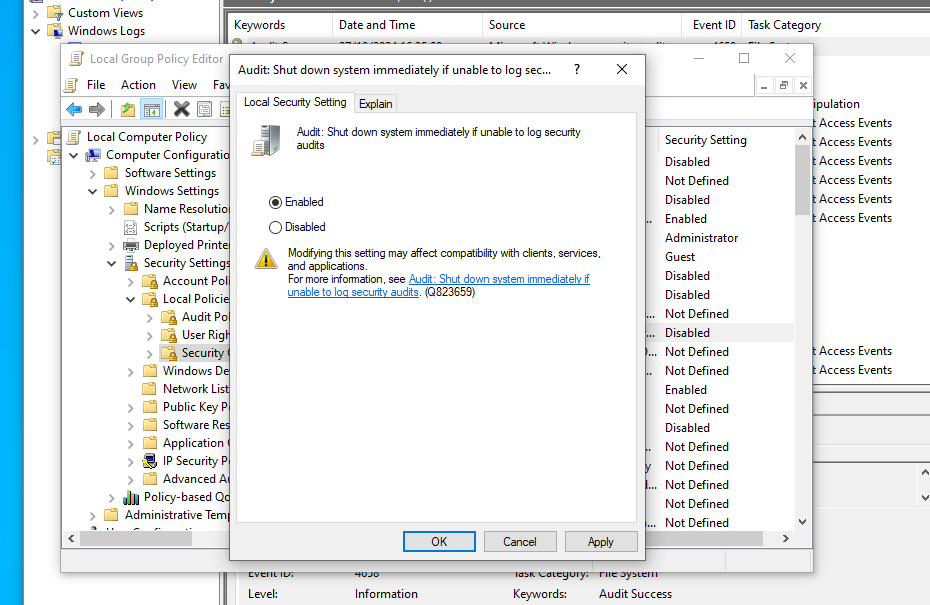
\includegraphics[width=\columnwidth]{5}
		\caption{Встановлення опції}
	\end{figure}
		\begin{figure}[H]
		\centering
		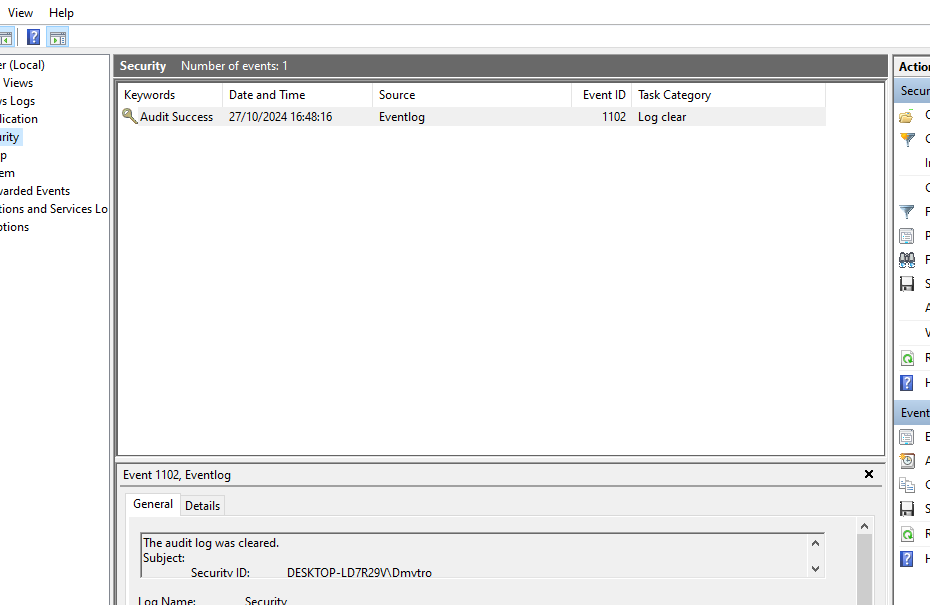
\includegraphics[width=\columnwidth]{6}
		\caption{Запис в журналі аудиту}
	\end{figure}
	\section*{Висновки}
	Під час виконання лабораторної роботи я ознайомився з політиками та налаштуванням аудиту,
	аналізом безпеки системи шляхом вивчення журналу подій в Windows 10.
	Навчився проводити аудит локальної системи та працювати з журналом
	безпеки Windows.
		    
\end{normalsize}
\end{document}
